\chapter{ANALYSE ET VÉRIFICATION DES PREMIERS RÉSULTATS}
\thispagestyle{empty}

\section{Analyse des résultats}

La branche révisée modifie de manière significative l'histoire du projet. Les
rapports précédents suggéraient que la récupération structurelle brute, en
particulier le Node2Vec non corrigé, constituait la direction la plus forte.
Après les corrections méthodologiques introduites dans la nouvelle branche, la
famille la plus performante est désormais la famille hybride corrigée :
\begin{itemize}
    \item \textbf{BGE pooled + Node2Vec (corrected)} obtient le meilleur score
    Hit@10, avec 0.0867.
    \item \textbf{BGE-M3 + Node2Vec (corrected)} est pratiquement à égalité sur
    Hit@10 et légèrement plus fort sur MRR, Recall et MAP.
\end{itemize}

Ce résultat est plus cohérent avec l'objectif réel du projet. Puisque le
système vise la recommandation d'articles plutôt que la simple complétion de
graphe, il est logique que les meilleurs modèles combinent similarité
sémantique et contexte structurel. La nouvelle branche conduit donc à une
conclusion plus équilibrée : la structure pure du graphe reste utile, mais la
fusion sémantique-structurelle apparaît désormais comme la direction la plus
convaincante pour le système final.

Un autre résultat important concerne le pooling. Dans la configuration de
concaténation précédente, BGE-M3 contribuait à hauteur de 1024 dimensions,
tandis que Node2Vec n'en contribuait que 128. Les nouveaux modèles avec
pooling compressent BGE-M3 à 128 dimensions avant concaténation. Cela ne
produit pas un saut spectaculaire, mais améliore légèrement le meilleur
résultat global sur Hit@10 et rend la représentation hybride équilibrée du
point de vue dimensionnel.

Une analyse sémantico-structurelle antérieure soutient également l'orientation
du projet à un niveau plus local. La Figure~\ref{fig:cosine-assortativity}
montre que les paires de nœuds liées tendent à avoir une similarité cosinus
plus élevée que les paires aléatoires. Ce résultat ne résout pas à lui seul le
problème de la recommandation, mais il vérifie que la similarité
textuelle-sémantique transporte un signal significatif aligné avec la
structure du graphe.

\begin{figure}[H]
\centering
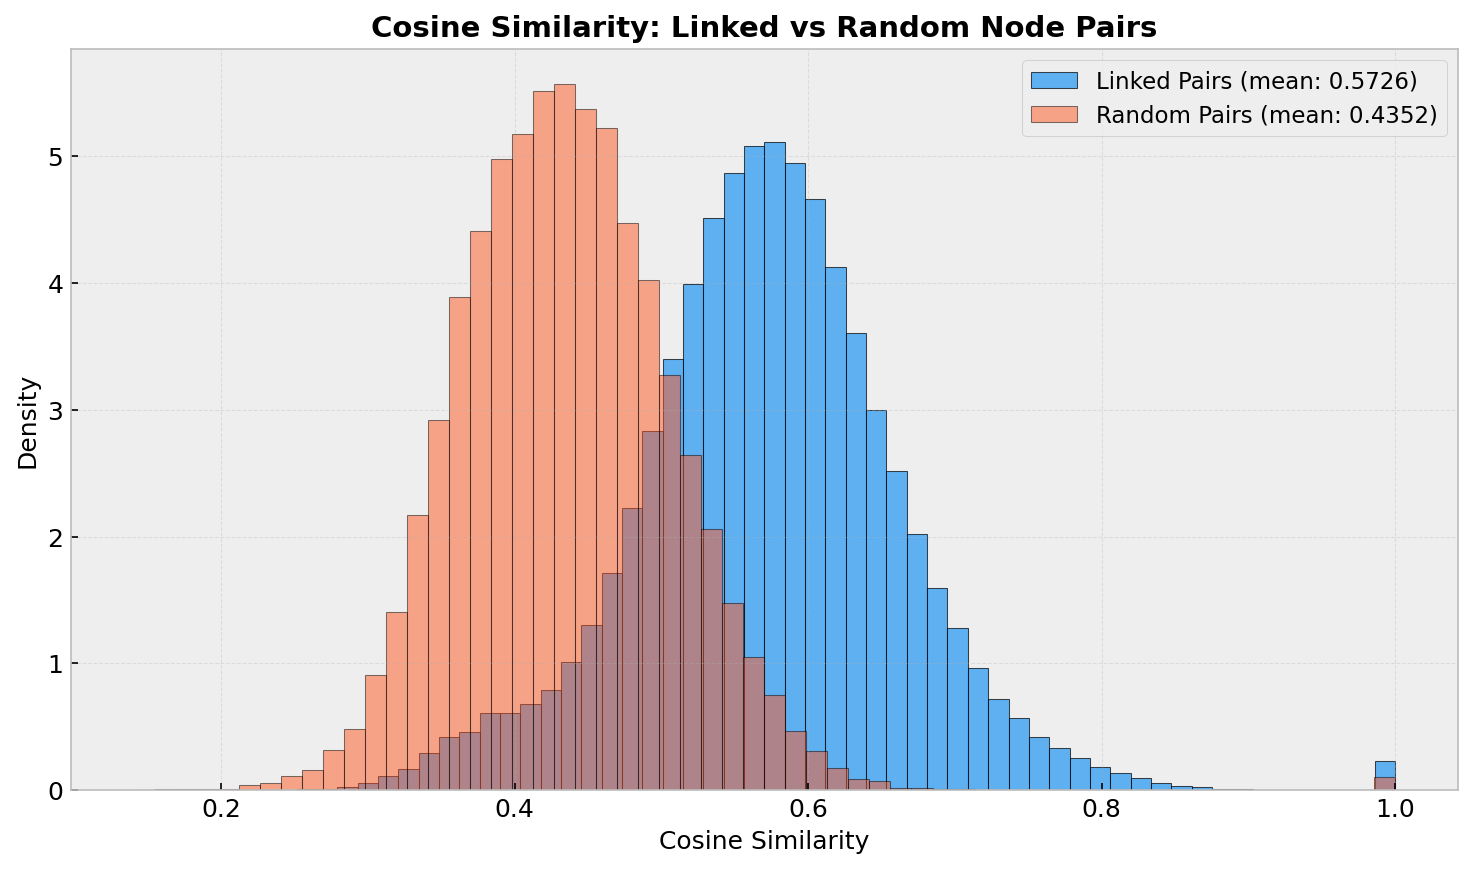
\includegraphics[width=0.82\textwidth]{figures/cosine-similarity-assortativity.png}
\caption{Distributions de similarité cosinus pour des paires de nœuds liées et pour des paires aléatoires. Les paires liées sont décalées vers des similarités plus élevées, ce qui indique que la proximité sémantique est informative pour la recommandation et l'évaluation.}
\label{fig:cosine-assortativity}
\end{figure}

Enfin, les métriques orientées recommandation révèlent un second axe de
qualité des modèles au-delà de la seule précision du classement. GCN Only
reste faible sur Hit@10 et MRR, mais il obtient de bons résultats sur des
métriques orientées diversité telles que Aggregate Diversity, Novelty et
Intra-List Distance. À l'inverse, BGE-M3 Only est davantage piloté par la
popularité. Les modèles hybrides corrigés occupent le compromis le plus utile :
ils conservent une qualité de classement compétitive tout en évitant les
formes les plus marquées de concentration sur des articles populaires.

\section{Tableaux de métriques étendus}

Pour être complet, la branche révisée inclut également le tableau combiné des
métriques et le résumé de classement par métrique qui avaient été assemblés
dans la série de rapports détaillés. Le
Tableau~\ref{tab:mid-combined-metrics-fr} reproduit les anciennes et nouvelles
métriques sur la branche à dix modèles, tandis que le
Tableau~\ref{tab:mid-rank-summary-fr} convertit ces valeurs brutes en rangs par
colonne afin de rendre la comparaison globale plus facile à lire.

\begin{table}[H]
\centering
\caption{Anciennes et nouvelles métriques combinées sur la branche révisée à dix modèles.}
\label{tab:mid-combined-metrics-fr}
\setlength{\tabcolsep}{3pt}
\renewcommand{\arraystretch}{1.12}
\resizebox{\textwidth}{!}{
\begin{tabular}{@{}>{\raggedright\arraybackslash}p{0.22\textwidth}*{13}{c}@{}}
\toprule
\textbf{Modèle} &
\textbf{H@1} &
\textbf{H@10} &
\textbf{H@50} &
\textbf{H@100} &
\textbf{MRR} &
\textbf{NDCG} &
\textbf{Recall} &
\textbf{MAP} &
\textbf{Pop. Lift} &
\textbf{Gini} &
\textbf{Agg. Div.} &
\textbf{Novelty} &
\textbf{ILD} \\
\midrule
BGE pooled + Node2Vec (corrected) & 1.03\% & 8.67\% & 31.46\% & 47.81\% & 0.0410 & 0.1160 & 0.4781 & 0.0392 & 1.3301 & 0.4110 & 11,326 & 14.2738 & 0.4372 \\
BGE-M3 + Node2Vec (corrected) & 1.07\% & 8.67\% & 32.41\% & 49.81\% & 0.0421 & 0.1202 & 0.4981 & 0.0403 & 1.3081 & 0.4127 & 11,268 & 14.2783 & 0.4316 \\
BGE pooled + Node2Vec (uncorrected) & 0.76\% & 7.83\% & 32.64\% & 50.74\% & 0.0376 & 0.1176 & 0.5074 & 0.0358 & 1.3397 & 0.4613 & 11,186 & 14.0351 & 0.4558 \\
BGE-M3 + Node2Vec (uncorrected) & 0.76\% & 7.83\% & 32.64\% & 50.74\% & 0.0376 & 0.1176 & 0.5074 & 0.0358 & 1.3400 & 0.4605 & 11,164 & 14.0340 & 0.4557 \\
Node2Vec (uncorrected) & 0.75\% & 7.81\% & 32.52\% & 50.60\% & 0.0375 & 0.1172 & 0.5060 & 0.0357 & 1.3374 & 0.4482 & 10,966 & 14.0466 & 0.4569 \\
Node2Vec (corrected) & 0.75\% & 7.81\% & 32.52\% & 50.60\% & 0.0375 & 0.1172 & 0.5060 & 0.0356 & 1.3374 & 0.4482 & 10,966 & 14.0466 & 0.4569 \\
GCN + BGE-M3 (rank fusion) & 0.85\% & 7.63\% & 23.14\% & 33.77\% & 0.0335 & 0.0862 & 0.3377 & 0.0317 & 1.6650 & 0.4228 & 11,655 & 13.9222 & 0.4366 \\
BGE-M3 Only & 1.35\% & 7.57\% & 19.69\% & 27.73\% & 0.0366 & 0.0788 & 0.2773 & 0.0351 & 1.9413 & 0.5172 & 10,905 & 13.8459 & 0.3713 \\
GCN Only & 0.38\% & 3.46\% & 14.12\% & 22.91\% & 0.0180 & 0.0530 & 0.2291 & 0.0163 & 1.1879 & 0.2607 & 11,685 & 14.3293 & 0.5135 \\
GraphSAGE Only & 0.17\% & 1.22\% & 4.96\% & 8.72\% & 0.0076 & 0.0199 & 0.0872 & 0.0061 & 1.3134 & 0.2517 & 11,628 & 14.2087 & 0.5313 \\
\bottomrule
\end{tabular}
}
\end{table}

\begin{table}[H]
\centering
\caption{Résumé des rangs par métrique sur la branche révisée à dix modèles. Un rang total plus faible est meilleur.}
\label{tab:mid-rank-summary-fr}
\setlength{\tabcolsep}{3pt}
\renewcommand{\arraystretch}{1.12}
\resizebox{\textwidth}{!}{
\begin{tabular}{@{}>{\raggedright\arraybackslash}p{0.22\textwidth}*{14}{c}@{}}
\toprule
\textbf{Modèle} &
\textbf{Total} &
\textbf{H@1} &
\textbf{H@10} &
\textbf{H@50} &
\textbf{H@100} &
\textbf{MRR} &
\textbf{NDCG} &
\textbf{Recall} &
\textbf{MAP} &
\textbf{Agg. Div.} &
\textbf{Novelty} &
\textbf{ILD} &
\textbf{Pop. Lift} &
\textbf{Gini} \\
\midrule
BGE-M3 + Node2Vec (corrected) & 1 & 2 & 2 & 5 & 5 & 1 & 1 & 5 & 1 & 5 & 2 & 9 & 2 & 4 \\
BGE pooled + Node2Vec (corrected) & 2 & 3 & 1 & 6 & 6 & 2 & 6 & 6 & 2 & 4 & 3 & 7 & 4 & 3 \\
BGE pooled + Node2Vec (uncorrected) & 3 & 6 & 3 & 1 & 1 & 4 & 3 & 1 & 4 & 6 & 7 & 5 & 7 & 9 \\
BGE-M3 + Node2Vec (uncorrected) & 4 & 5 & 4 & 2 & 2 & 3 & 2 & 2 & 3 & 7 & 8 & 6 & 8 & 8 \\
Node2Vec (uncorrected) & 5 & 7 & 5 & 3 & 3 & 5 & 4 & 3 & 5 & 8 & 5 & 3 & 5 & 6 \\
Node2Vec (corrected) & 6 & 8 & 6 & 3 & 3 & 6 & 5 & 3 & 6 & 8 & 5 & 3 & 5 & 6 \\
GCN Only & 7 & 9 & 9 & 9 & 9 & 9 & 9 & 9 & 9 & 1 & 1 & 2 & 1 & 2 \\
GCN + BGE-M3 (rank fusion) & 8 & 4 & 7 & 7 & 7 & 8 & 7 & 7 & 8 & 2 & 9 & 8 & 9 & 5 \\
GraphSAGE Only & 9 & 10 & 10 & 10 & 10 & 10 & 10 & 10 & 10 & 3 & 4 & 1 & 3 & 1 \\
BGE-M3 Only & 10 & 1 & 8 & 8 & 8 & 7 & 8 & 8 & 7 & 10 & 10 & 10 & 10 & 10 \\
\bottomrule
\end{tabular}
}
\end{table}

\section{Vérification et contrôles de cohérence}

Les résultats actuels n'ont pas été acceptés tels quels ; ils ont été
vérifiés et corrigés à plusieurs reprises au cours du développement. Les
principales étapes de vérification ont été les suivantes :
\begin{itemize}
    \item validation des statistiques de la séparation révisée de phase 0 :
    216\,123 arêtes non orientées, 172\,900 arêtes d'entraînement, 43\,223
    arêtes de test, et aucun nouveau nœud isolé introduit par la séparation,
    \item réestimation du coefficient structurel de loi de puissance sur la
    branche révisée, donnant $\alpha \approx 2.9966$,
    \item séparation des informations de validation et de test pendant
    l'entraînement de GCN et GraphSAGE sur la branche révisée,
    \item vérification de cohérence entre les notebooks, les caches générés et
    les tableaux finaux de résultats inclus dans les rapports,
    \item correction de problèmes antérieurs liés à l'état des notebooks, y
    compris un fichier notebook JSON mal formé et des résultats mis en cache
    devenus obsolètes.
\end{itemize}

La branche révisée clarifie aussi un problème qui affectait l'interprétation
de la lignée report-6. À cette étape antérieure, une mise de côté orientée des
arêtes sortantes était combinée avec une modélisation structurelle qui
consommait finalement un graphe non orienté, en particulier dans la famille
Node2Vec. Cela créait un risque de fuite ou, au minimum, un décalage
méthodologique : le modèle pouvait bénéficier d'une vue structurelle qui ne
respectait pas pleinement la définition orientée du holdout. En conséquence,
certaines conclusions antérieures, notamment la domination apparente du
Node2Vec brut, ont dû être considérées avec prudence et réévaluées
explicitement dans la branche non orientée révisée.

Les bases de référence GNN ont également été vérifiées indépendamment à
travers leurs valeurs d'AUC de test en prédiction de liens sur la branche
révisée :
\begin{table}[H]
\centering
\caption{Résultats de vérification des GNN structurels sur la branche révisée.}
\label{tab:gnn-auc}
\begin{tabular}{lc}
\toprule
\textbf{Modèle} & \textbf{AUC de test} \\
\midrule
GCN Only & 0.9304 \\
GraphSAGE Only & 0.9190 \\
\bottomrule
\end{tabular}
\end{table}

Ces valeurs d'AUC confirment que les deux bases de référence GNN structurelles
apprennent une structure de graphe non triviale, même si leurs performances en
classement de recommandation restent inférieures à celles des meilleurs modèles
hybrides. Dans l'ensemble, la branche actuelle peut donc être considérée à la
fois comme empiriquement informative et techniquement vérifiée.
